\section{Solution \#2:}

The \textbf{updated} storyboard for this solution:\\
(we updated the storyboard to be fun for both parent and child)

\begin{figure}[H]
	\centering
	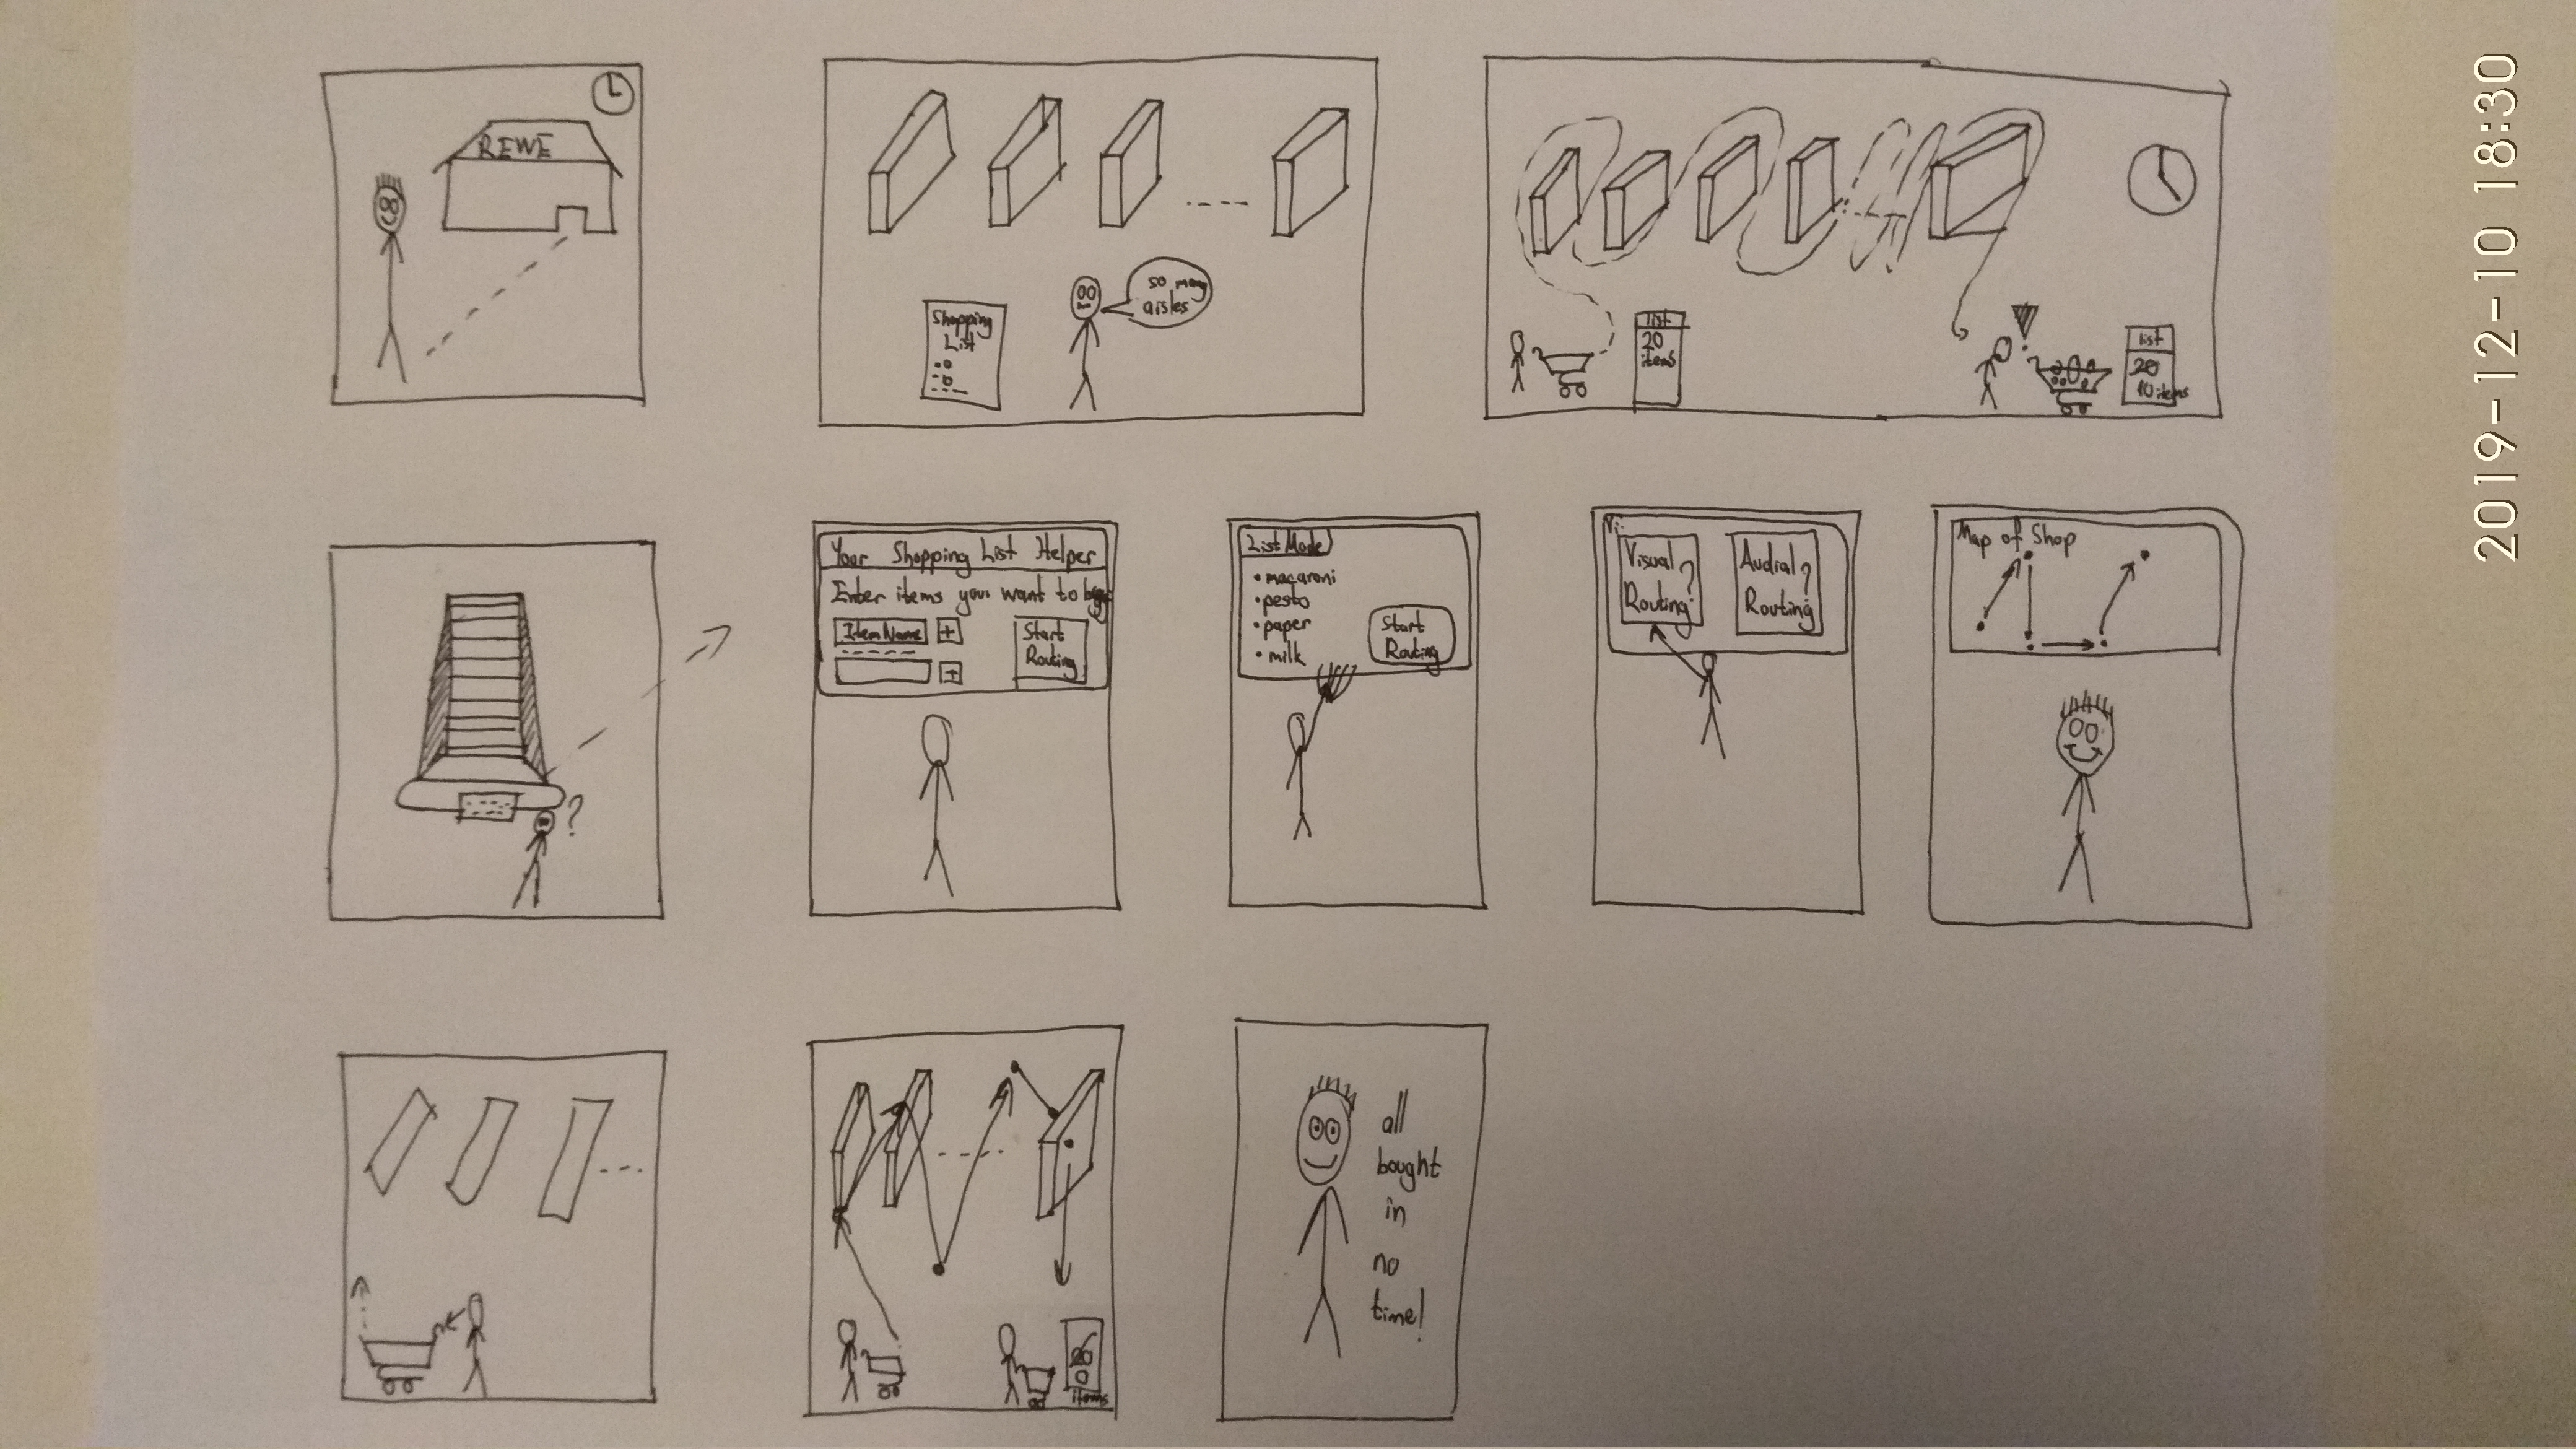
\includegraphics[trim={0em 10em 10em 10em}, clip, scale=0.5, width=0.90\textwidth]{images/s2/2/s1.jpg}
\end{figure}

\subsection{Core Activities of this Solution}

\begin{itemize}
	\item creating a shopping list
	
%	\item barcode scanning
	
	\item choose a coutry user wants to "visit"
\end{itemize}

\subsection{The Reason for Prototype Selection}

It's an mobile app which is not complex and all the parts of the screens are changing so we choosed simple paper prototype.

\subsection{Rough prototypes}
\begin{figure}[H]
	\centering
	\includegraphics[trim={0em 10em 10em 10em}, angle=270, clip, scale=0.5, width=0.40\textwidth]{images/s2/2/rough/1.jpg}
\end{figure}

\begin{figure}[H]
	\centering
	\includegraphics[trim={10em 20em 10em 20em}, clip, width=0.60\textwidth]{images/s2/2/rough/2.jpg}
\end{figure}



\subsection{Prototyping Process Explained}

All of us created some rough types, than we met and merged them into one and improved it. Our screens are:
\begin{itemize}
	\item welcome screen\\
	(\autoref{s2:menu} )
	
	\item menu about shoping lists\\
	(\autoref{s2:lists} )
	\begin{enumerate}
		\item recommendations
		\begin{itemize}
     		\item Viewing a shoping list
     		(\autoref{s2:shoplist} )
   		\end{itemize}
    	\item shopping without a list
    	\item creating a shoping list
    	(\autoref{s2:with} )
    	\begin{itemize}
     		\item viewing a shoping list
     		(\autoref{s2:shoplist} )
   		\end{itemize}
	\end{enumerate}
	
	\item menu about selecting a country\\
	(\autoref{s2:countrylist} )
	\begin{itemize}
     	\item randomly choosed country
     	\item user selects country
     	(\autoref{s2:selectcountry} )
   	\end{itemize}
   	
   	\item ending screen\\
   	(\autoref{s2:end} )
	
\end{itemize}

\clearpage
\subsection{Prototype Itself}

\begin{figure}[H]
	\centering
	\includegraphics[trim={10em 10em 10em 10em}, angle=270, clip, width=0.90\textwidth]{images/s2/1/1.jpg}
	\caption{ The Welcome Screen }
	\label{s2:menu}
\end{figure}

\begin{figure}[H]
	\centering
	\includegraphics[trim={10em 10em 10em 10em}, angle=270, clip, width=0.9\textwidth]{images/s2/1/3.jpg}
	\caption{ Menu about shoping lists}
	\label{s2:lists}
\end{figure}

\begin{figure}[H]
	\centering
	\includegraphics[trim={10em 10em 10em 10em}, angle=270, clip, width=0.9\textwidth]{images/s2/3/3.jpg}
	\caption{User chooses products that he wants to buy}
	\label{s2:with}
\end{figure}

\begin{figure}[H]
	\centering
	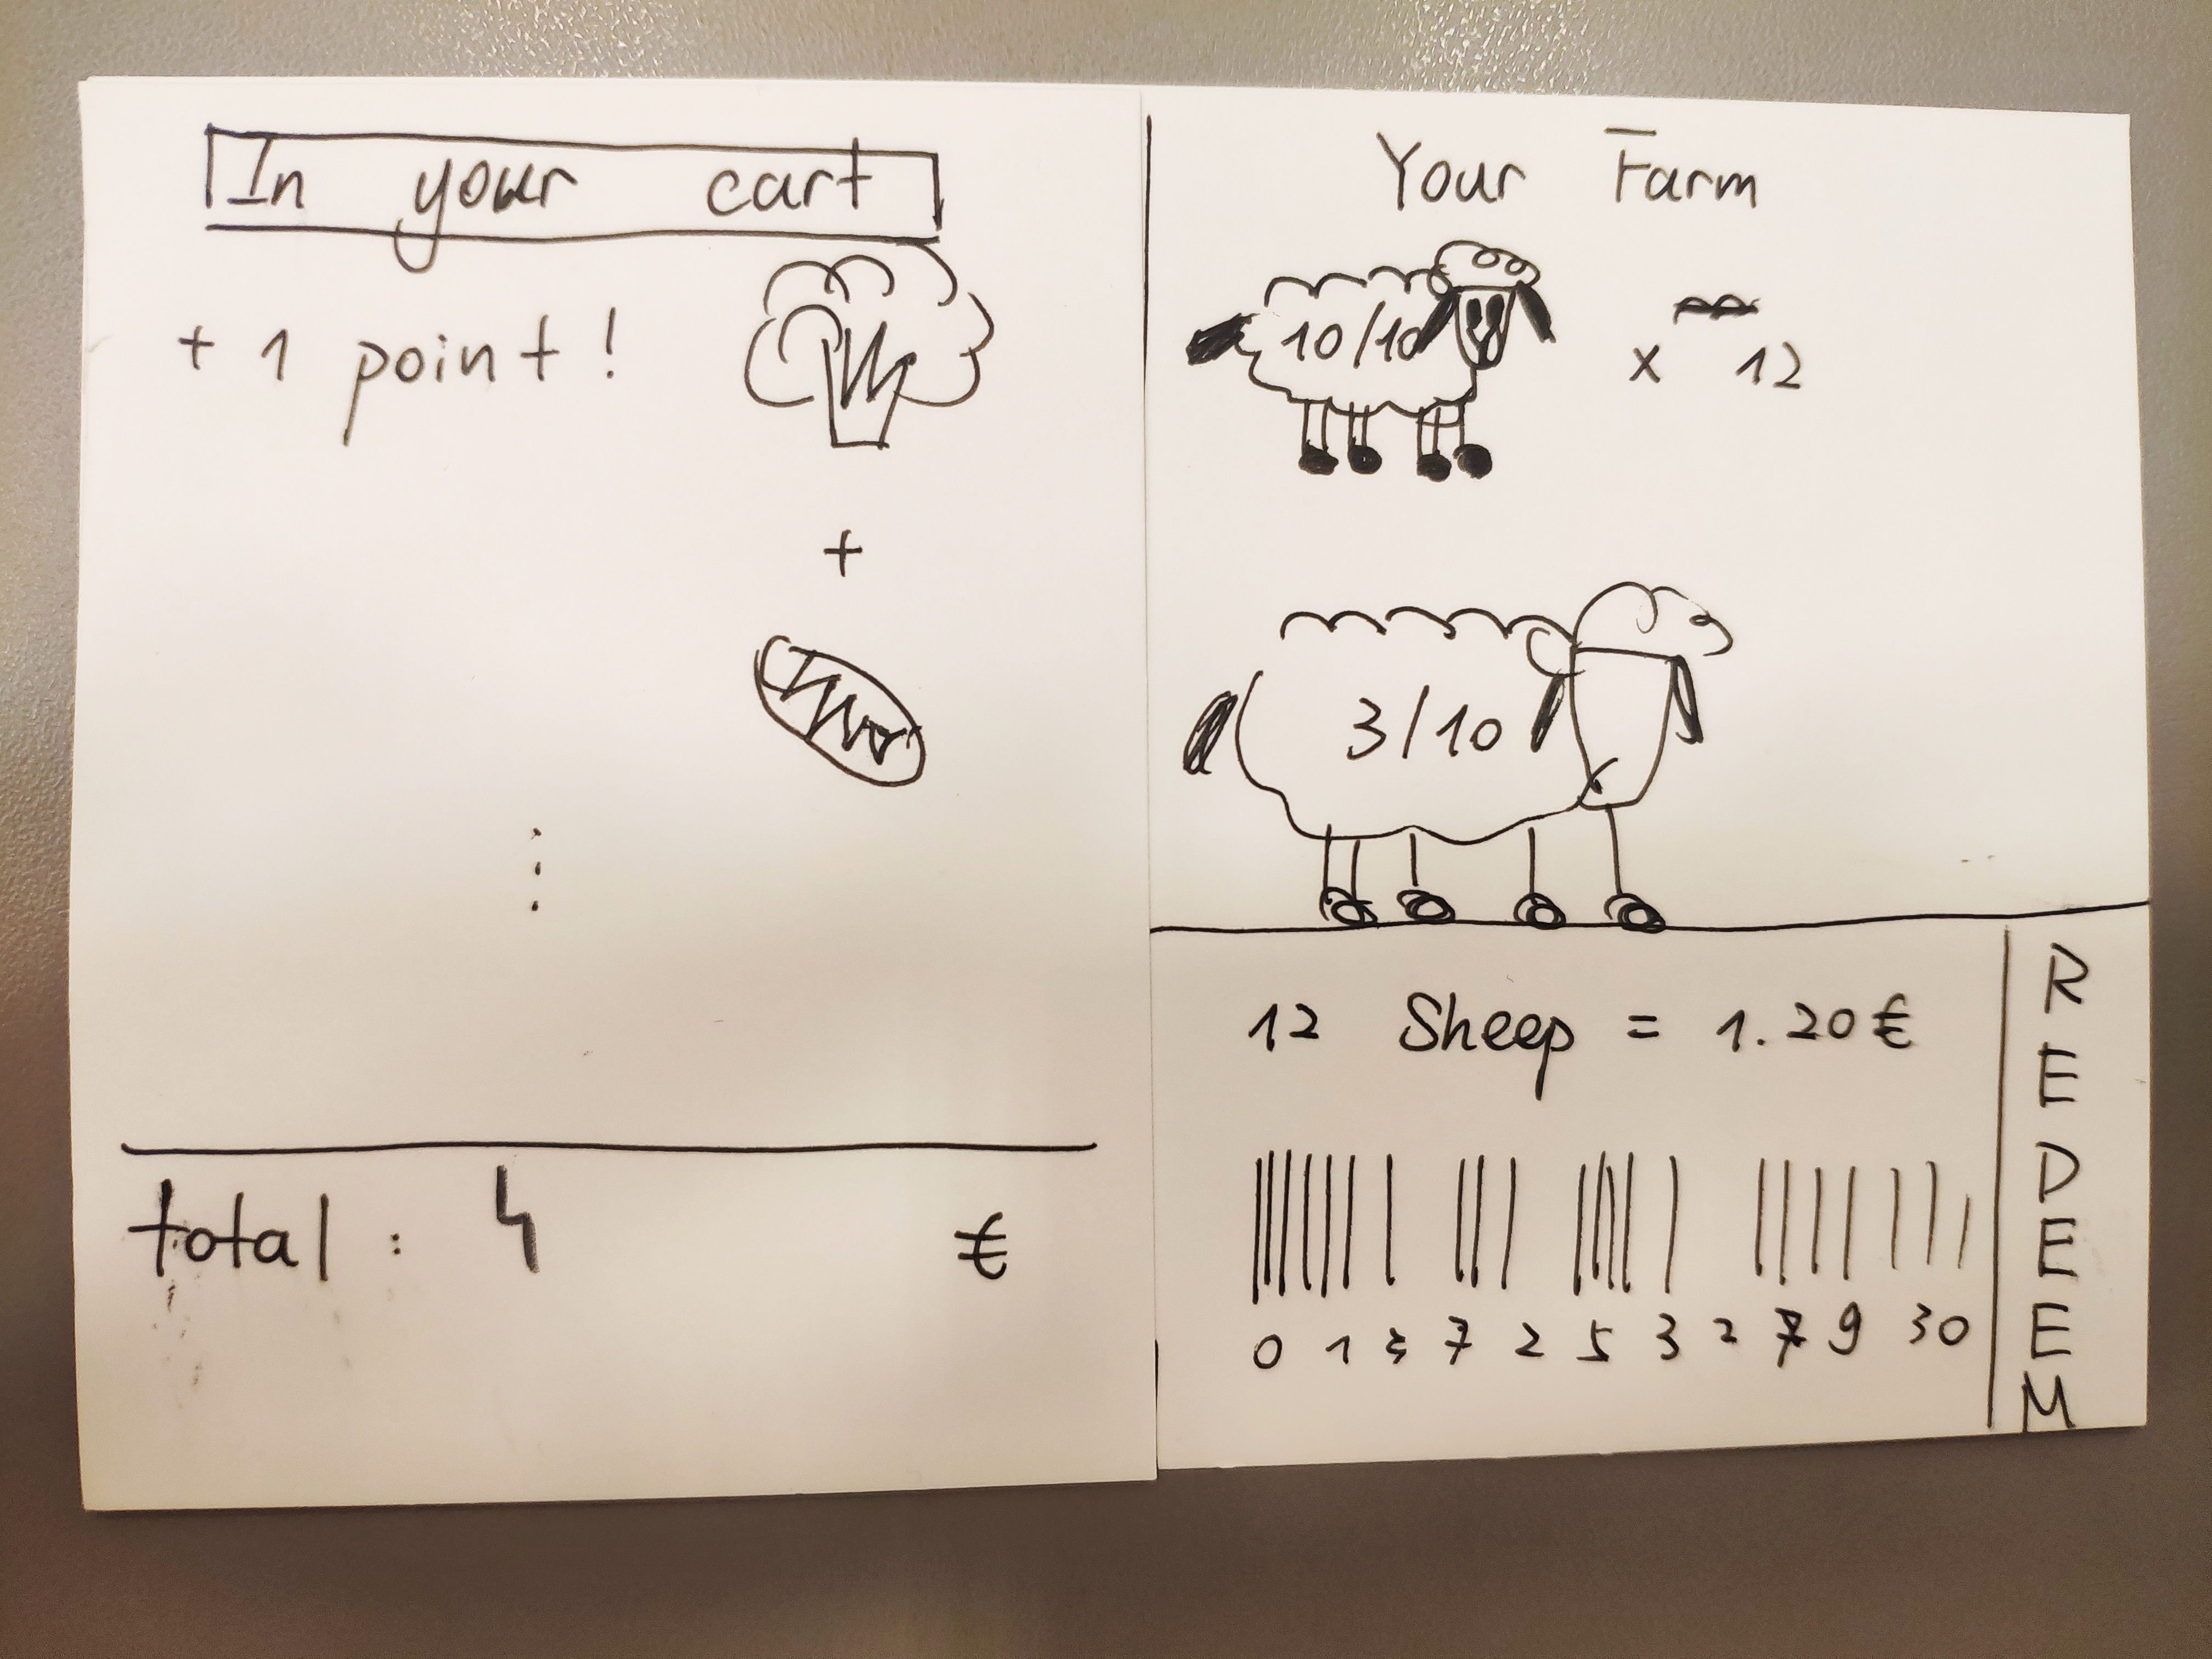
\includegraphics[trim={10em 10em 10em 10em}, angle=270, clip, width=0.9\textwidth]{images/s2/1/5.jpg}
	\caption{User views the shoping list}
	\label{s2:shoplist}
\end{figure}

\begin{figure}[H]
	\centering
	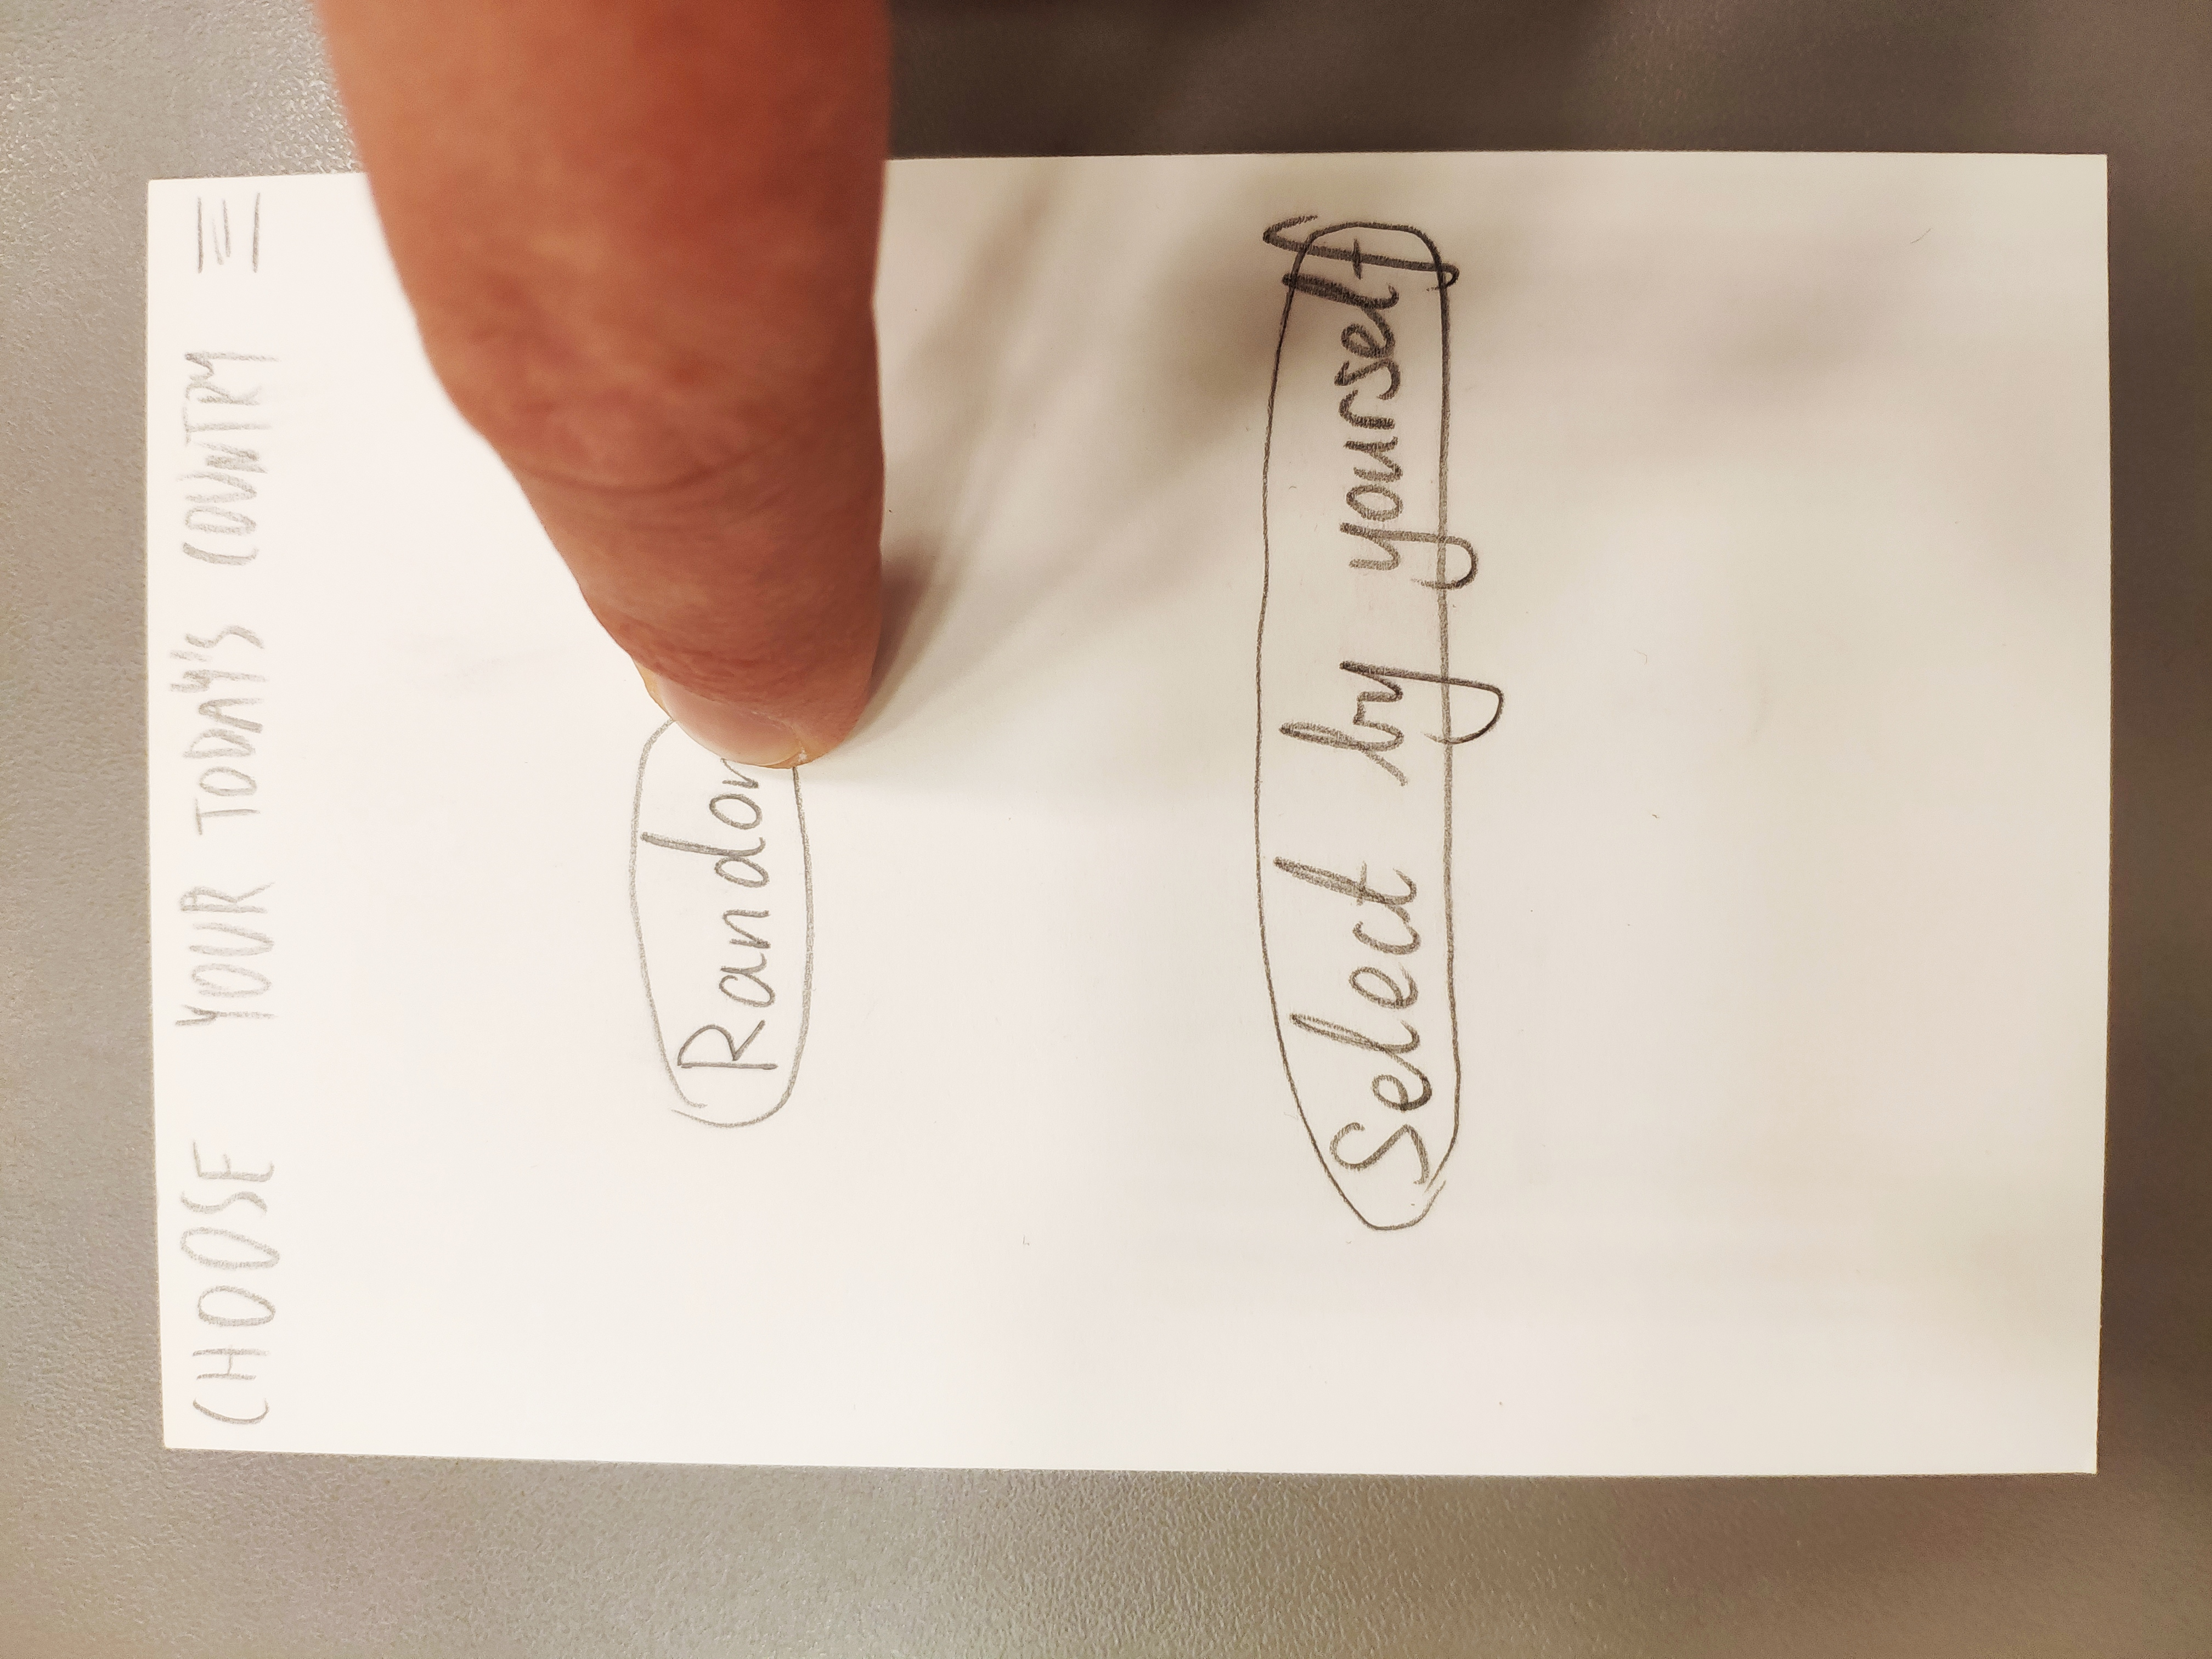
\includegraphics[trim={10em 10em 10em 10em}, angle=270, clip, width=0.9\textwidth]{images/s2/1/7.jpg}
	\caption{User selects if he wants to go to random country or choose by himself}
	\label{s2:countrylist}
\end{figure}

\begin{figure}[H]
	\centering
	\includegraphics[trim={10em 10em 10em 10em}, angle=270, clip, width=0.9\textwidth]{images/s2/2/4.jpg}
	\caption{User selects country to go}
	\label{s2:selectcountry}
\end{figure}


\begin{figure}[H]
	\centering
	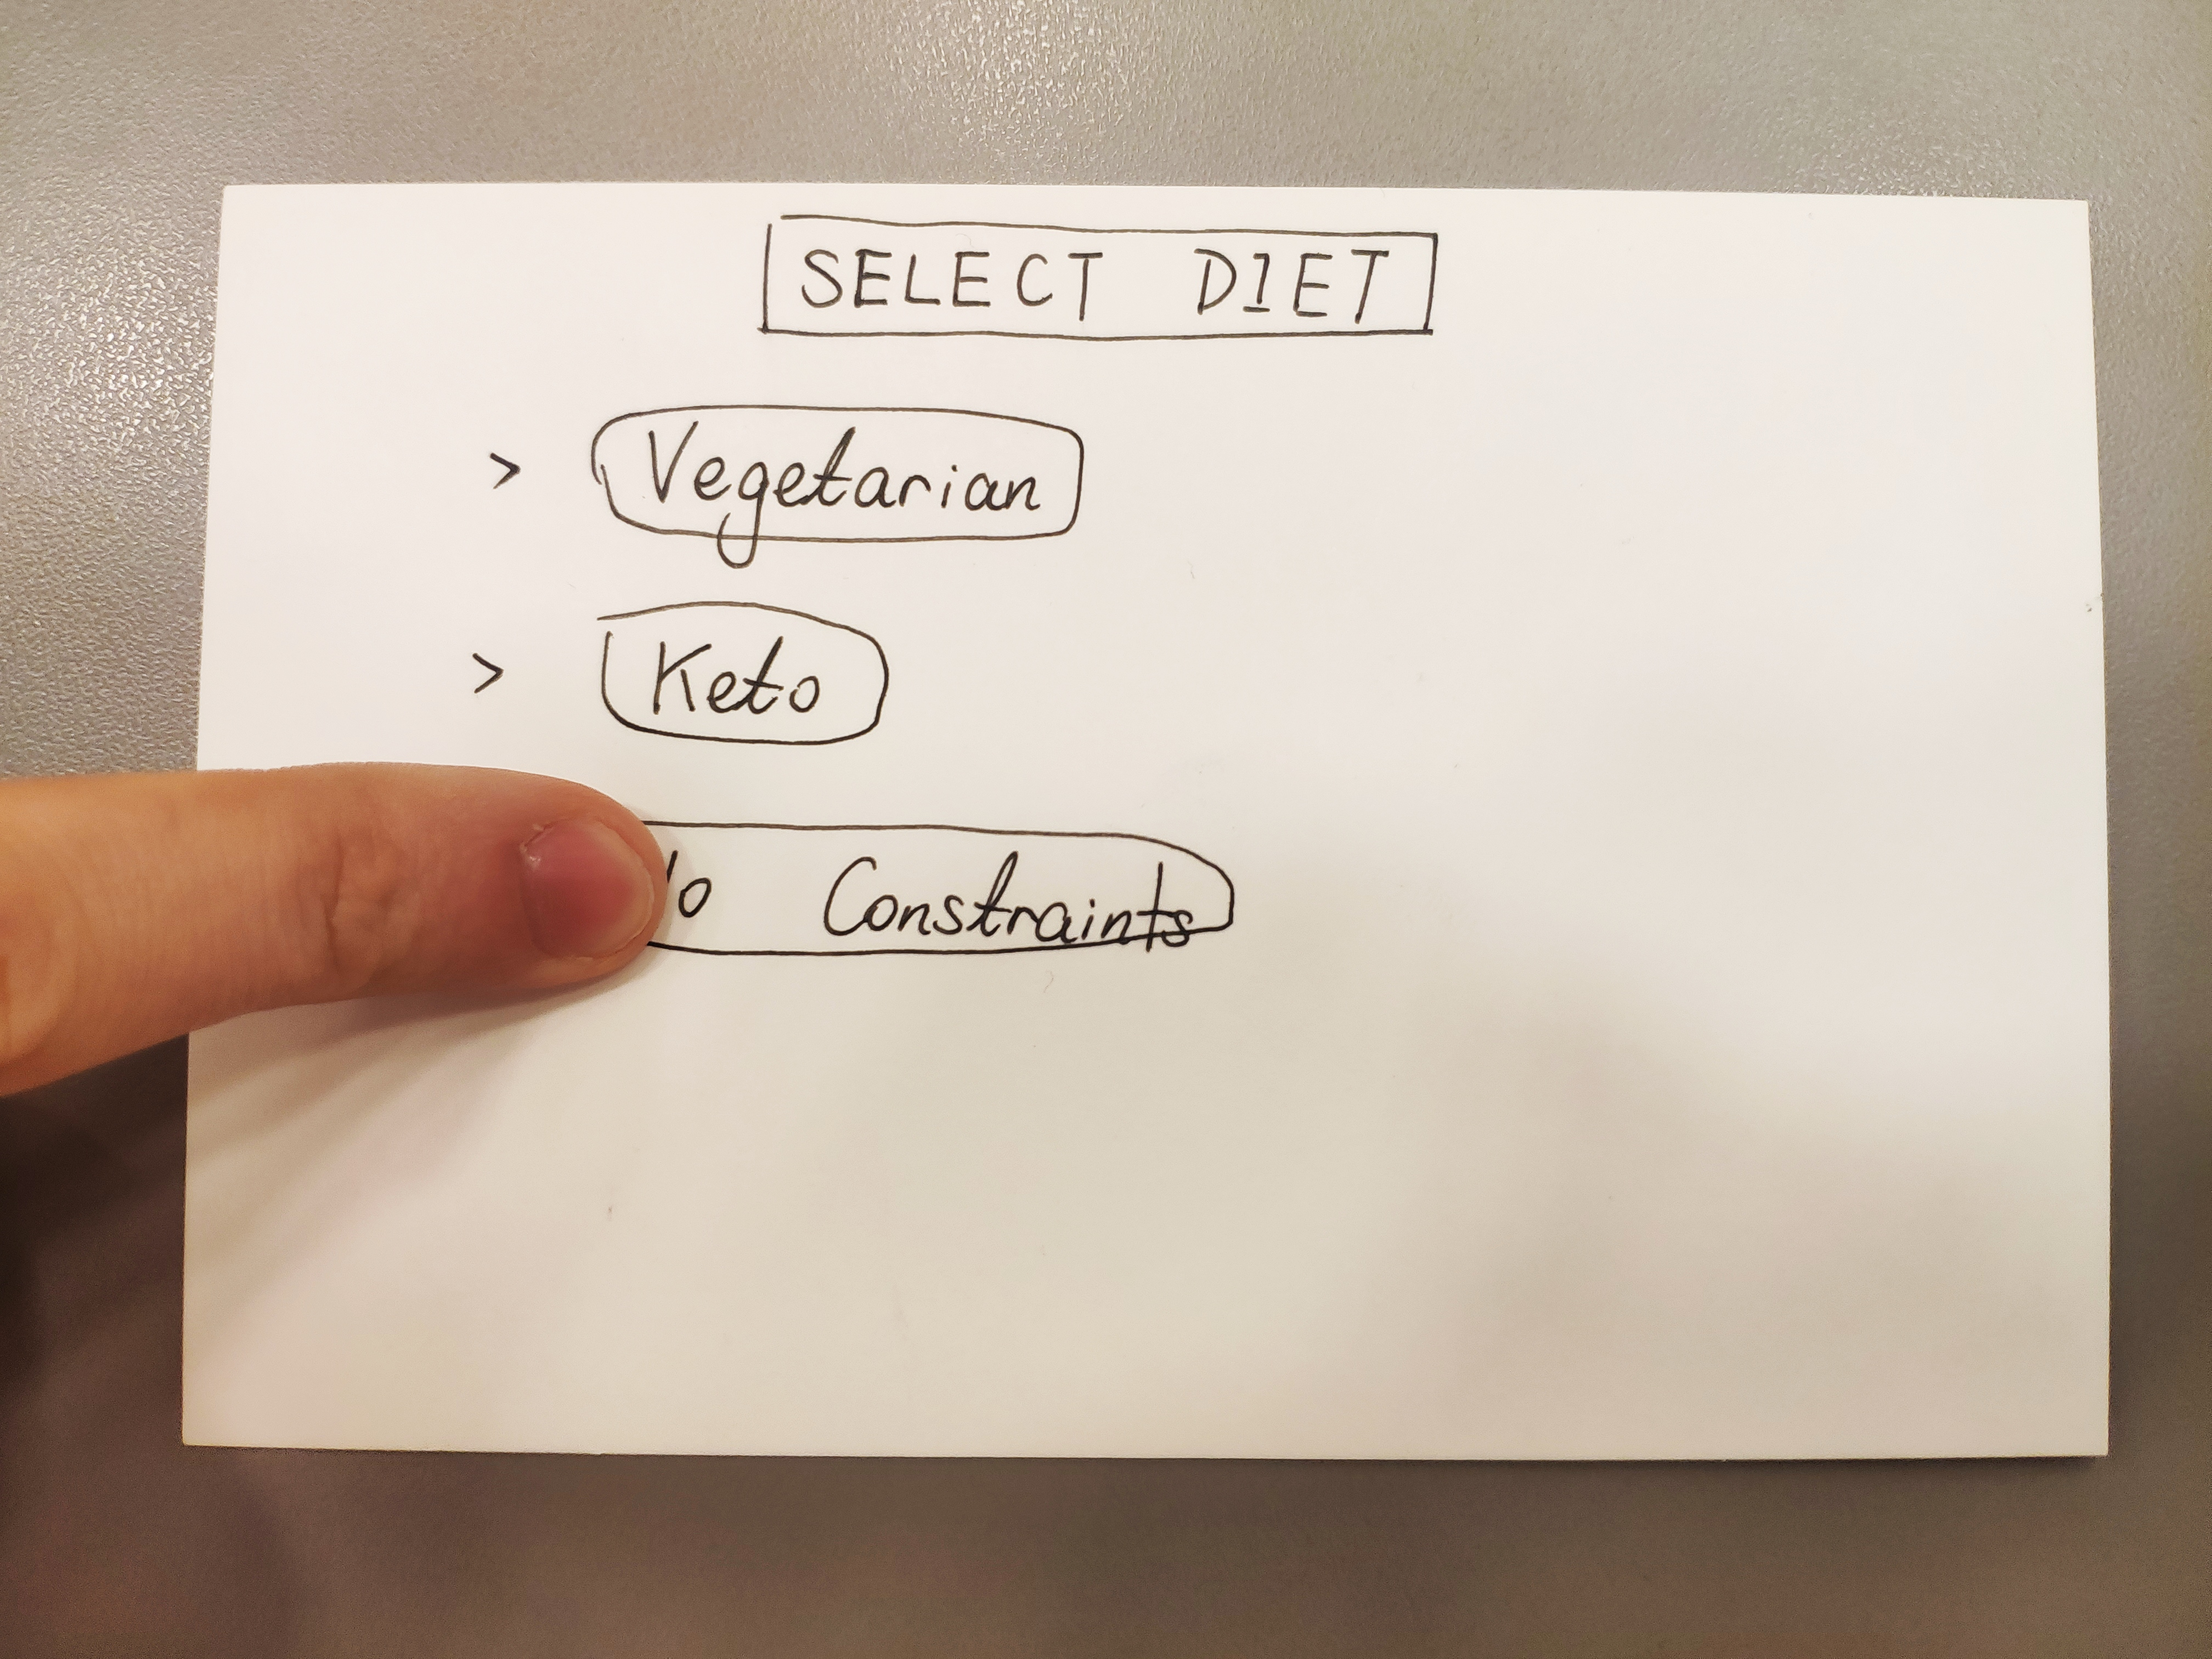
\includegraphics[trim={10em 10em 10em 10em}, angle=270, clip, width=0.9\textwidth]{images/s2/1/9.jpg}
	\caption{Screen with information about country}
	\label{s2:end}
\end{figure}